
\documentclass[11pt]{exam} % https://www.ctan.org/pkg/exam?lang=en

\usepackage[lmargin=1.in,rmargin=1.in,tmargin=1.in,bmargin=1in]{geometry}
\usepackage{setspace}
\usepackage[pdftex]{graphicx}
\usepackage{titling}
\usepackage[
	pdfauthor={Brian Weinstein},
	pdftitle={Homework 1},
	bookmarks=true,
	colorlinks=true,
	linkcolor=blue,
	urlcolor=blue,
	citecolor=blue,
	pdftex,
	linktocpage=true
	]{hyperref}
\usepackage[textsize=tiny]{todonotes}
\usepackage{float}
\setlength\parindent{0pt}
\usepackage{lipsum}
\usepackage{amsmath}
\usepackage{caption}


\qformat{\textbf{Problem \thequestion: \thequestiontitle}\quad \hfill}


\pagestyle{headandfoot}
\runningheadrule
\firstpageheader{}{}{}
\runningheader{\theauthor}{\thetitle}{\thedate}
\firstpagefooter{}{\thepage}{}
\runningfooter{}{\thepage}{}


\usepackage{xcolor}
\usepackage{adjustbox}
\usepackage{verbatim}
\definecolor{shadecolor}{rgb}{.9, .9, .9}

\newenvironment{code}%
   {\par\noindent\adjustbox{margin=1ex,bgcolor=shadecolor,margin=0ex \medskipamount}\bgroup\minipage\linewidth\verbatim}%
   {\endverbatim\endminipage\egroup}

\newenvironment{codeSmall}%
   {\par\noindent\adjustbox{margin=1ex,bgcolor=shadecolor,margin=0ex \medskipamount}\bgroup\minipage\linewidth\verbatim\footnotesize}%
   {\endverbatim\endminipage\egroup}

\newcommand{\ramsey}{\href{http://www.statisticalsleuth.com/}{Ramsey }}



\begin{document}


\title{STAT W4201 001, Homework 6}
\author{Brian Weinstein (bmw2148)}
\date{Mar 9, 2016}
\maketitle

Code is attached here and also posted at \href{https://github.com/BrianWeinstein/advanced-data-analysis}{https://github.com/BrianWeinstein/advanced-data-analysis}. Where relevant, code snippets and output are are included in-line.

\begin{questions}


\titledquestion{\ramsey 9.14}

\begin{parts}

\part \textit{Draw a matrix of scatterplots of the four variables. Construct it so that the bottom row of plots all have heart on the vertical axis. If you do not have this facility, draw scatterplots of heart versus each of the other variables individually.}

A matrix of pairwise scatterplots is shown in Figure \ref{fig:1a}.

\begin{figure}[!h]
	\centering
	\captionsetup{width=0.8\textwidth}
	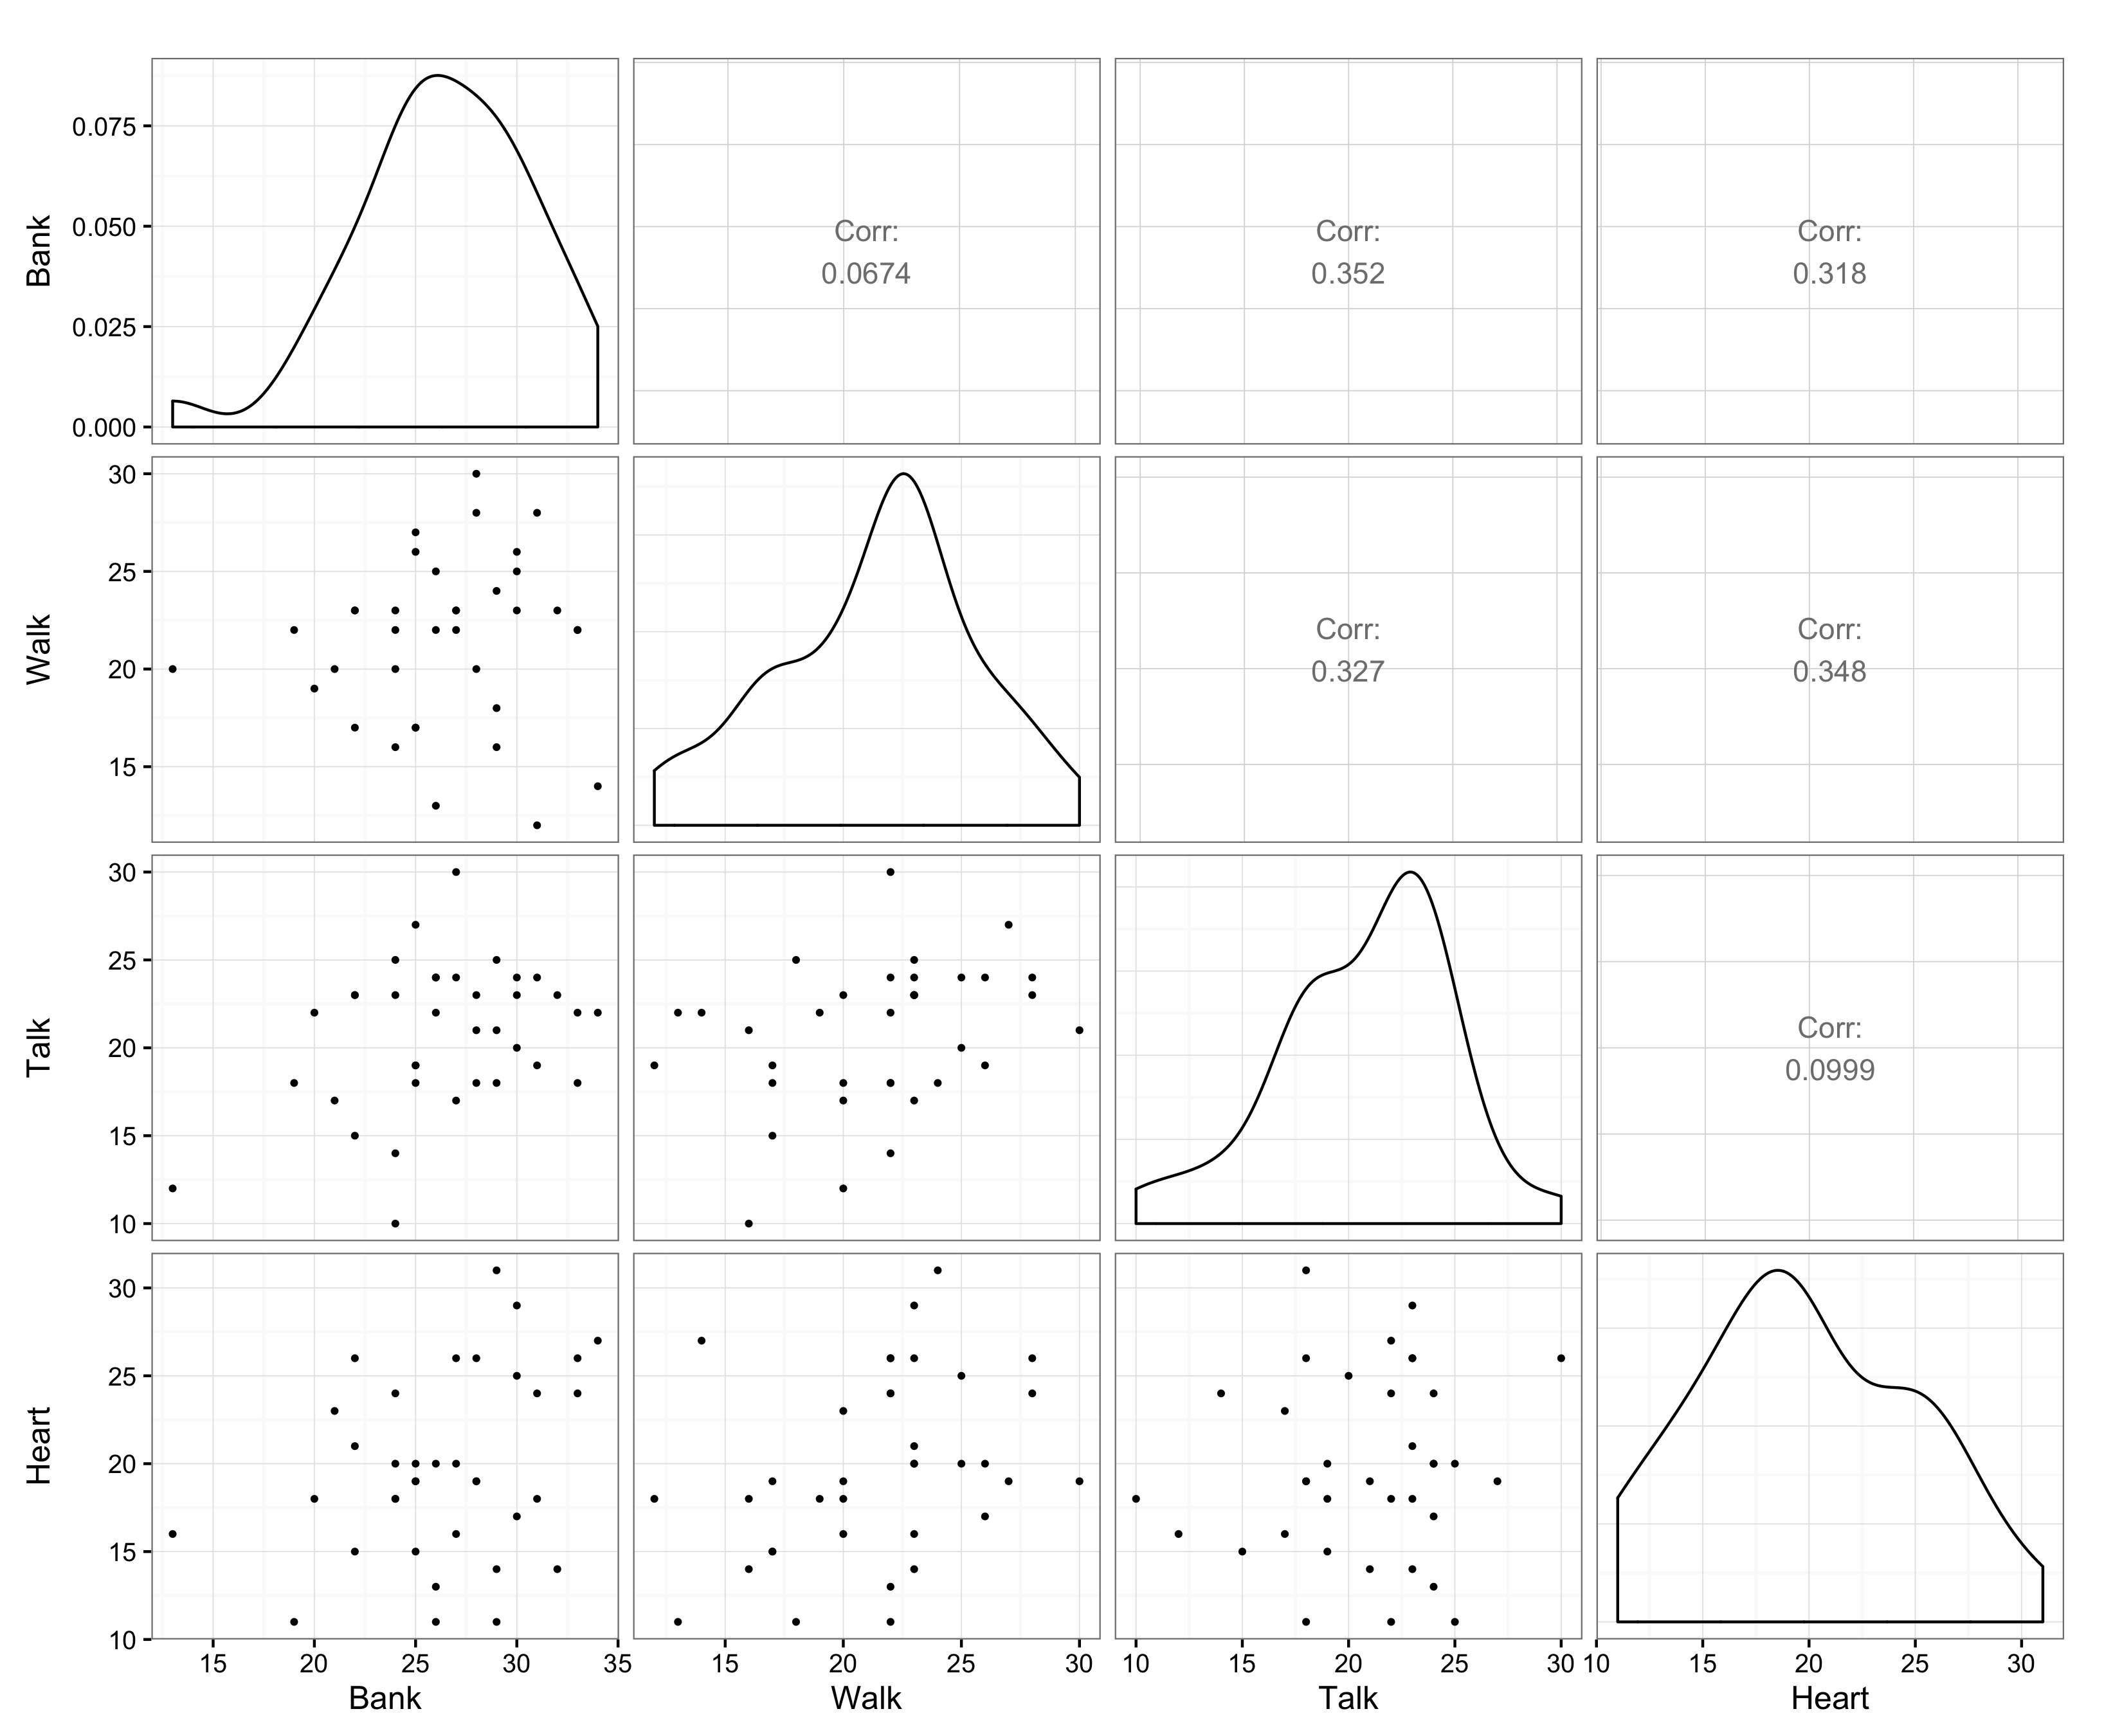
\includegraphics[width=\textwidth]{1a.png}
	\caption{Pairwise scatterplots of the variables in the ``Pace of Life and Heart Disease'' dataset.}
	\label{fig:1a}
\end{figure}

\part \textit{Obtain the least squares fit to the linear regression of heart on bank, walk, and talk.} \label{prob:0914b}

\begin{codeSmall}
> lmPace <- lm(formula=Heart ~ Bank + Walk + Talk, data=paceData)
> summary(lmPace)

Call:
lm(formula = Heart ~ Bank + Walk + Talk, data = paceData)

Residuals:
    Min      1Q  Median      3Q     Max 
-8.4014 -3.0263  0.0602  2.6748  8.4646 

Coefficients:
            Estimate Std. Error t value Pr(>|t|)  
(Intercept)   3.1787     6.3369   0.502   0.6194  
Bank          0.4052     0.1971   2.056   0.0480 *
Walk          0.4516     0.2009   2.248   0.0316 *
Talk         -0.1796     0.2222  -0.808   0.4249  
---
Signif. codes:  0 ‘***’ 0.001 ‘**’ 0.01 ‘*’ 0.05 ‘.’ 0.1 ‘ ’ 1

Residual standard error: 4.805 on 32 degrees of freedom
Multiple R-squared:  0.2236,	Adjusted R-squared:  0.1509 
F-statistic: 3.073 on 3 and 32 DF,  p-value: 0.04162
\end{codeSmall}

\part \textit{Plot the residuals versus the fitted values. Is there evidence that the variance of the residuals increases with increasing fitted values or that there are any outliers?}

The residual plot is shown in Figure \ref{fig:1c}. There does not seem to be evidence that the variance of the residuals increases with increasing fitted values, or that there are any extreme outliers.

\begin{figure}[!h]
	\centering
	\captionsetup{width=0.8\textwidth}
	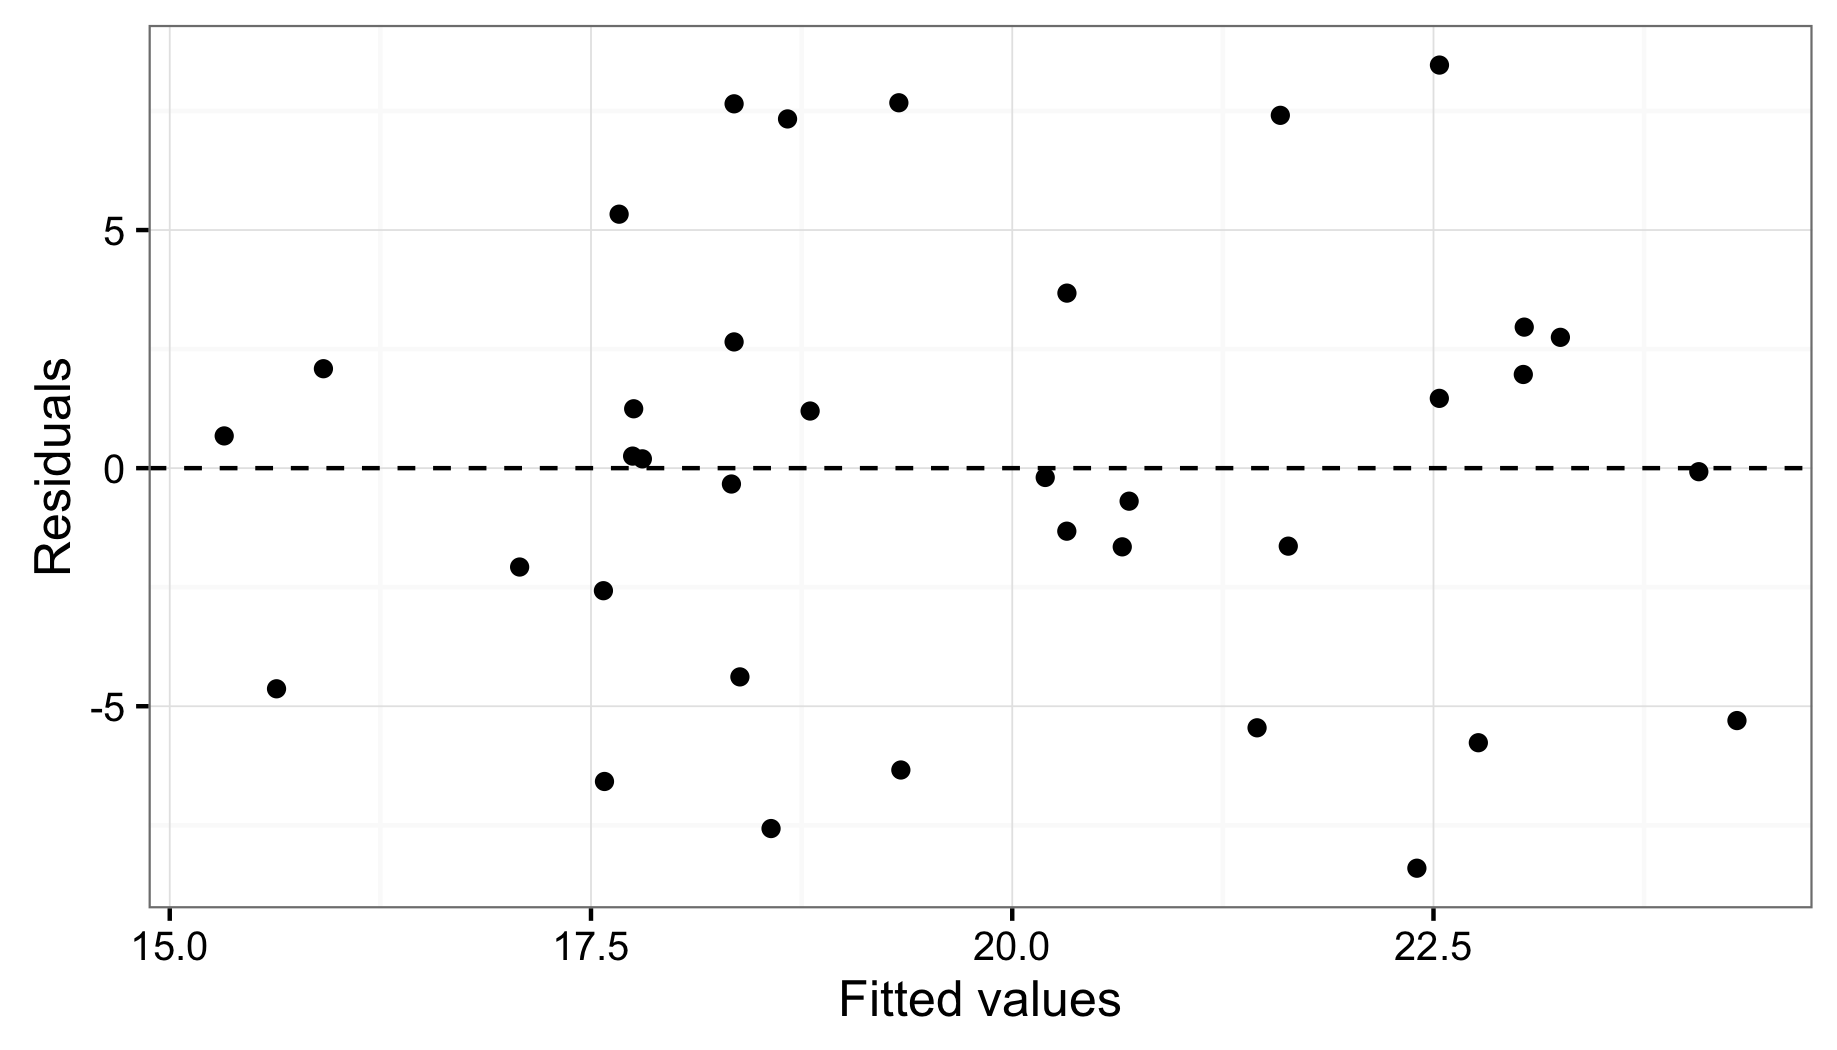
\includegraphics[width=4.25in]{1c.png}
	\caption{Residual plot for the fitted model from part (\ref{prob:0914b}).}
	\label{fig:1c}
\end{figure}

\part \textit{Report a summary of the least squares fit. Write down the estimated equation with standard errors below each estimated coefficient.}

Under the parallel lines regression model, the age-adjusted death rate due to heart disease (\texttt{Heart}) increases by $0.4052$ for every one unit increase in the bank clerk speed (\texttt{Bank}) (95\% confidence interval from $0.0037$ to $0.8067$). Similarly, \texttt{Heart} increases by $.4516$ for every one unit increase in the pedestrian walking speed (\texttt{Walk}) (95\% confidence interval from $0.0424$ to $0.8608$). The data provides no evidence that \texttt{Heart} is associated with postal clerk talking speed (\texttt{Talk}) (two sided p-value = $0.4249$ for a test that the \texttt{Talk} coefficient is zero).

The estimated equation is:
\begin{align*}
\mu\{\texttt{Heart}|\texttt{Bank}, \texttt{Walk}, \texttt{Talk}\} = &3.1787 + &&0.4052 \cdot \texttt{Bank} + &&0.4516 \cdot \texttt{Walk} + &&(-0.1796) \cdot \texttt{Talk} \\
&(6.3369) &&(0.1971) &&(0.2009) &&(0.2222)
\end{align*}

\end{parts}




\titledquestion{\ramsey 9.16}

\begin{parts}

\part \textit{Draw a coded scatterplot of proportion of pollen removed versus duration of visit; use different symbols or letters as the plotting codes for queens and workers. Does it appear that the relationship between proportion removed and duration is a straight line?}

A scatterplot of proportion of pollen removed versus duration of visit, by bee type is shown in Figure \ref{fig:2a}. It does not appear that the relationship between proportion removed and duration is a straight line.

\begin{figure}[!h]
	\centering
	\captionsetup{width=0.8\textwidth}
	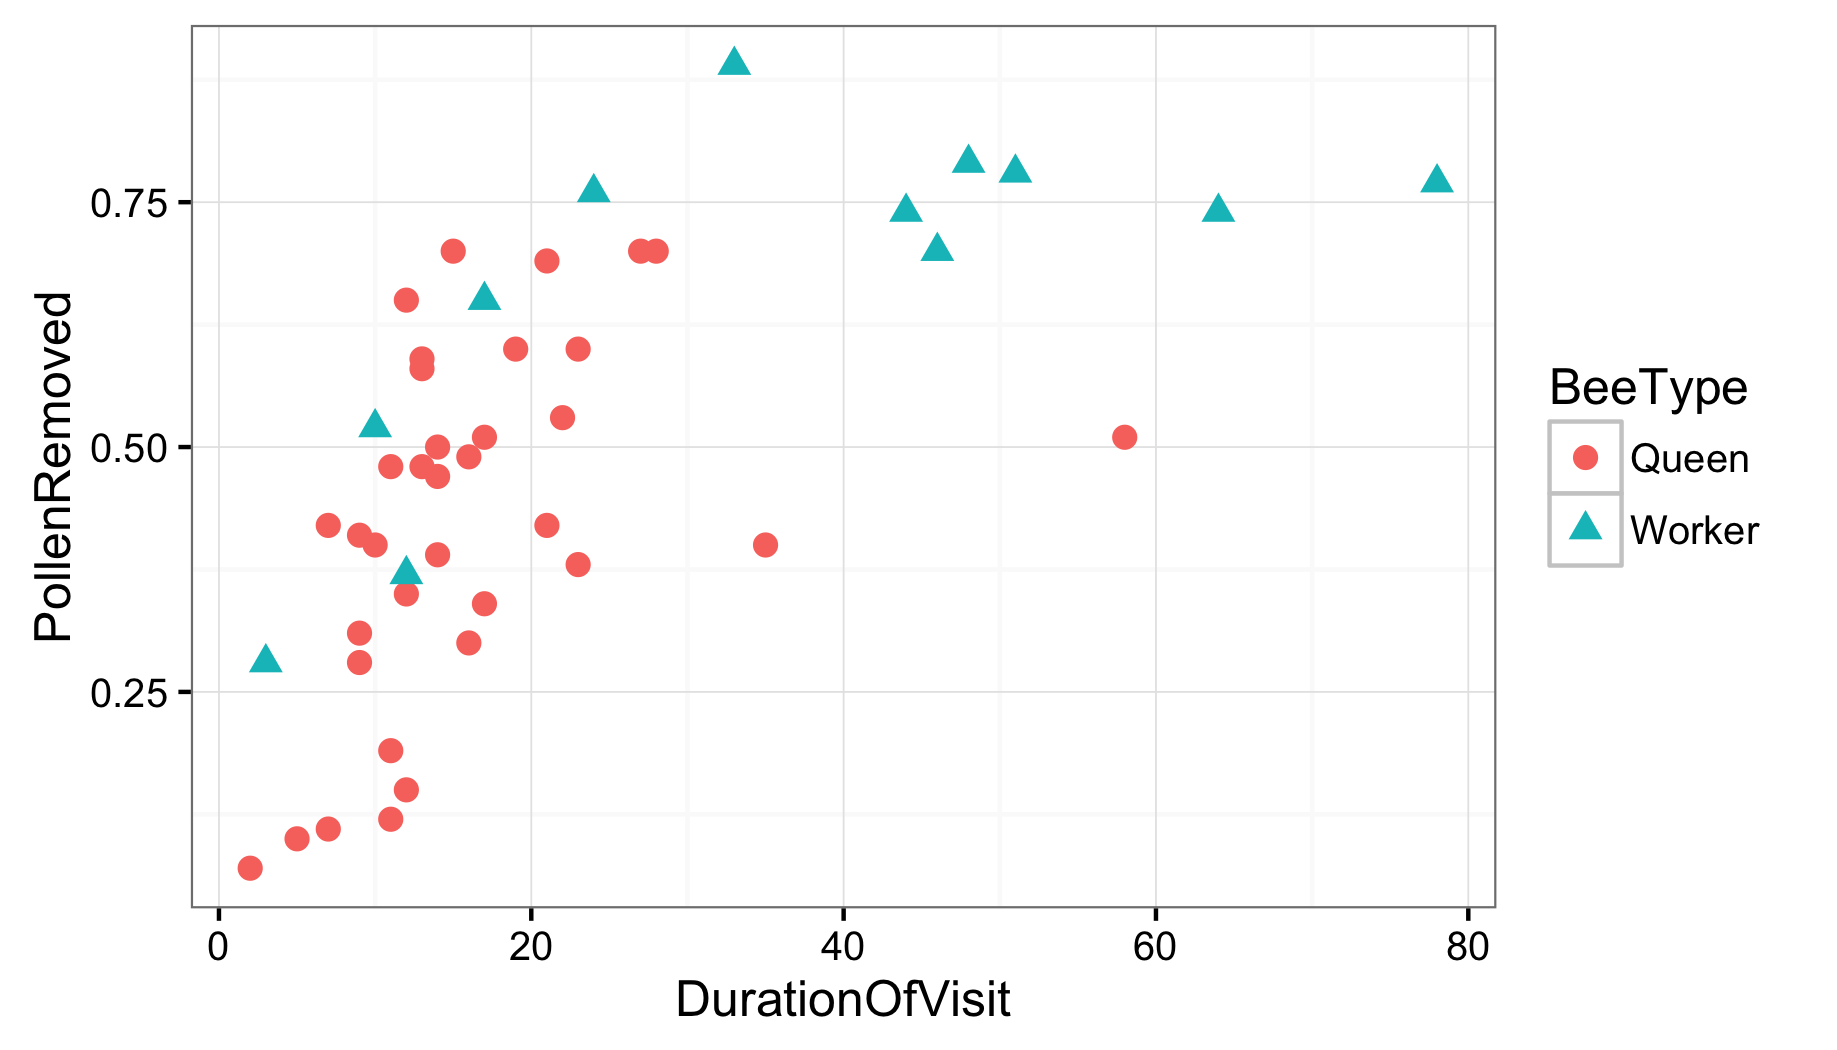
\includegraphics[width=4.25in]{2a.png}
	\caption{Scatterplot of pollen removed versus duration of visit, by bee type.}
	\label{fig:2a}
\end{figure}

\part \textit{The logit transformation is often useful for proportions between 0 and 1. If p is the proportion then the logit is $\log[p/(1-p)]$. This is the log of the ratio of the amount of pollen removed to the amount not removed. Draw a coded scatterplot of the logit versus duration.}

A scatterplot of the logit of proportion of pollen removed versus duration of visit, by bee type is shown in Figure \ref{fig:2b}.

\begin{figure}[!h]
	\centering
	\captionsetup{width=0.8\textwidth}
	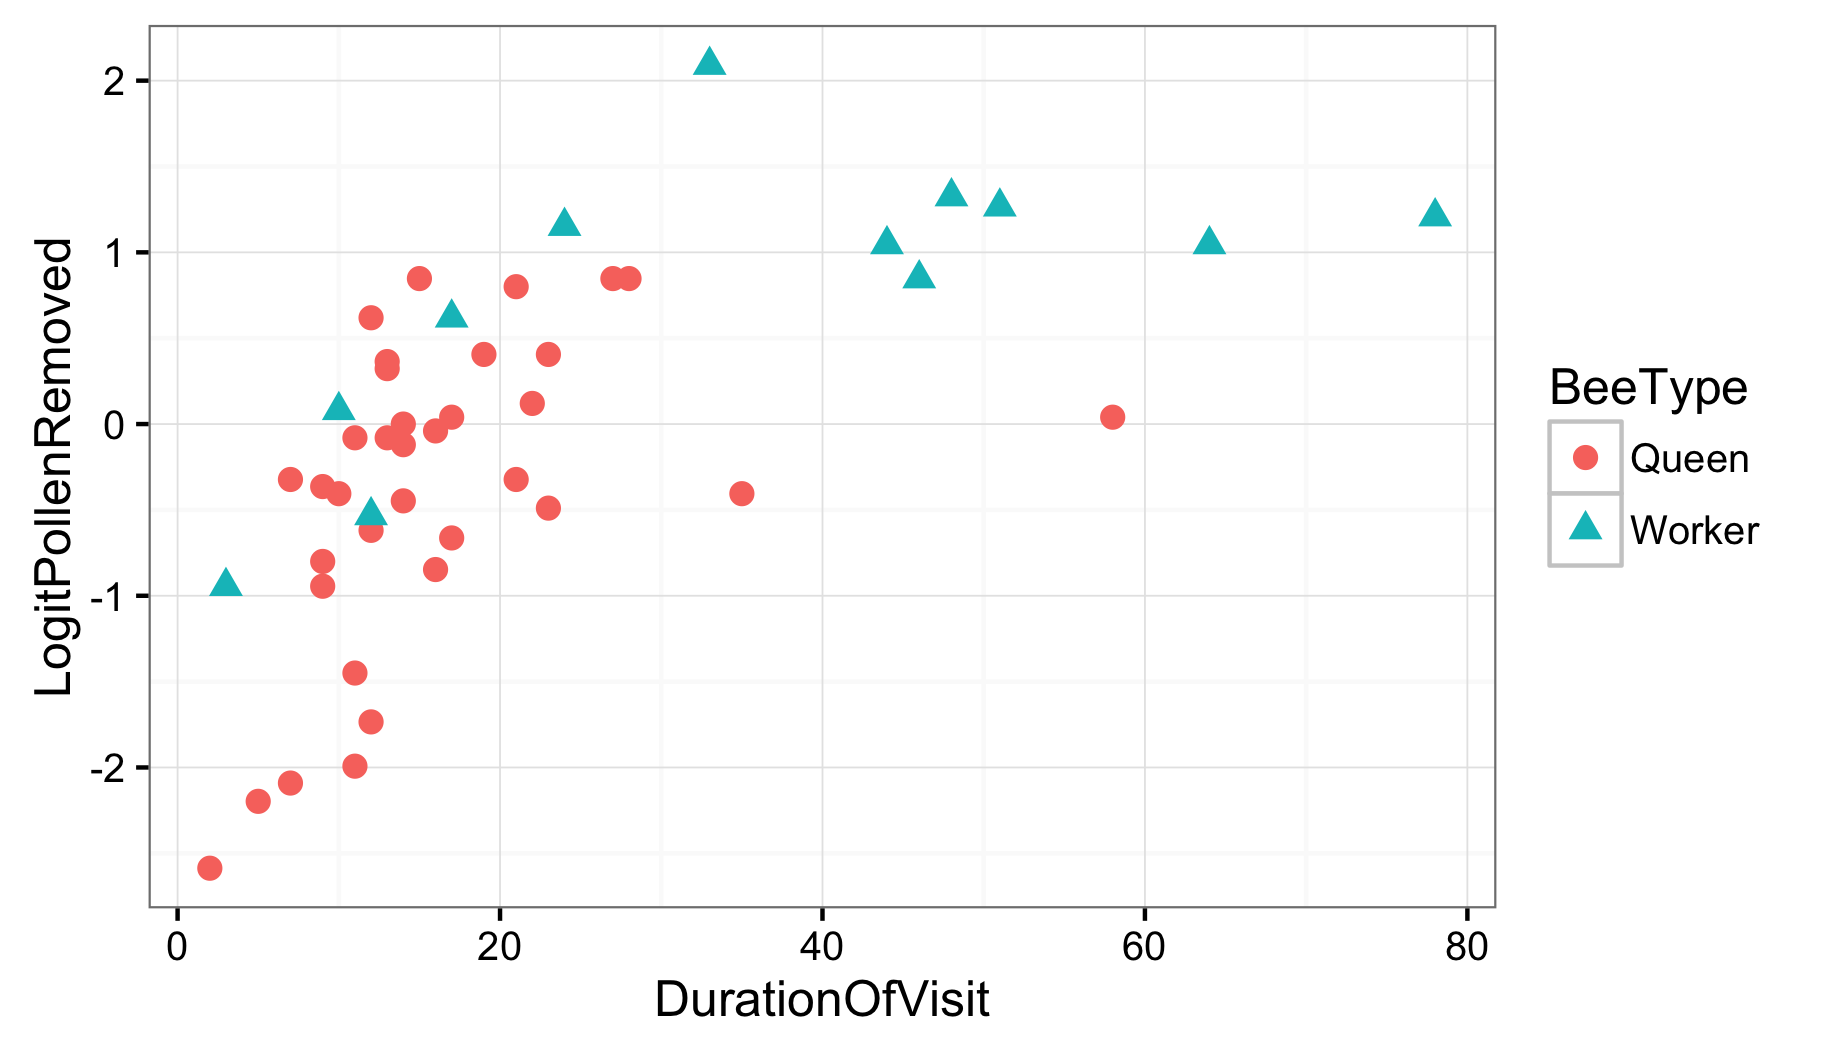
\includegraphics[width=4.25in]{2b.png}
	\caption{Scatterplot of the logit of pollen removed versus duration of visit, by bee type.}
	\label{fig:2b}
\end{figure}


\part \textit{Draw a coded scatterplot of the logit versus log duration. From the three plots, which transformations appear to be worthy of pursuing with a regression model?}

A scatterplot of the logit of proportion of pollen removed versus the log duration of visit, by bee type is shown in Figure \ref{fig:2c}. The Logit(PollenRemoved) vs Log(DurationOfVisit) transformations produce the most linear relationship, and is worthy of pursuing with a regression model.

\begin{figure}[!h]
	\centering
	\captionsetup{width=0.8\textwidth}
	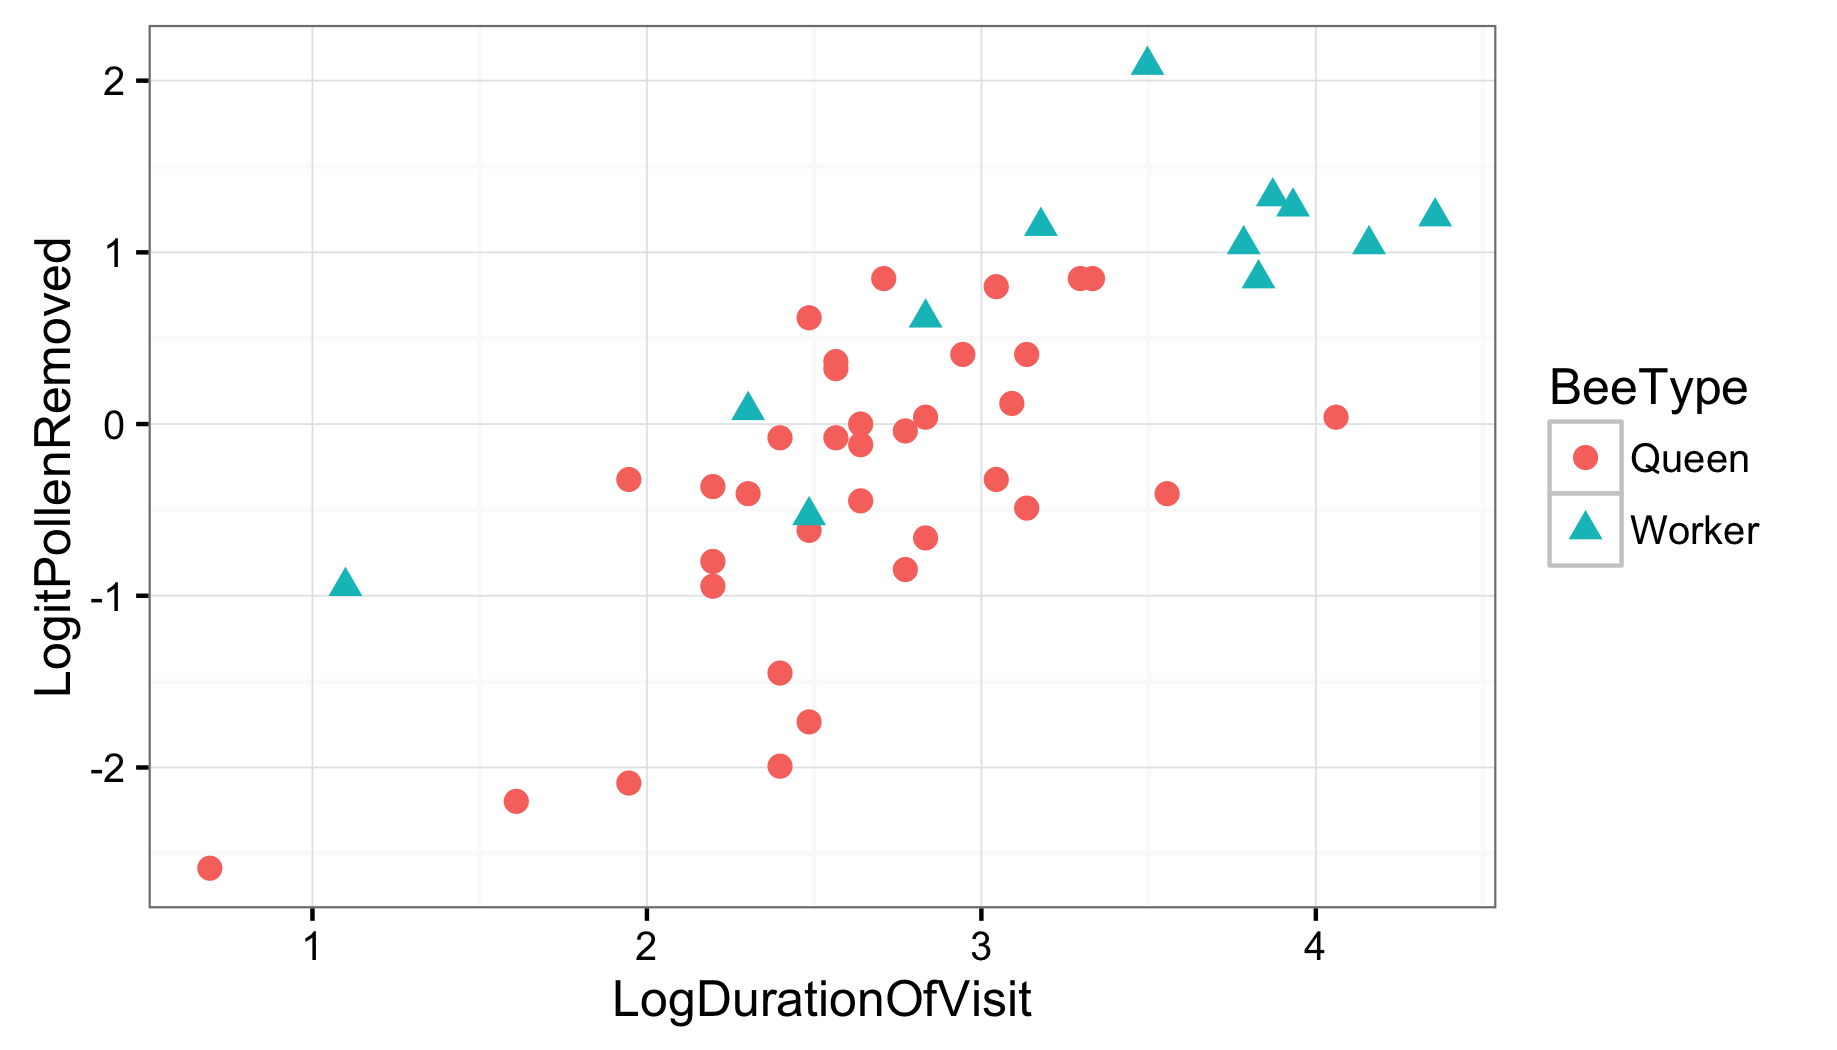
\includegraphics[width=4.25in]{2c.png}
	\caption{Scatterplot of the logit of pollen removed versus the log duration of visit, by bee type.}
	\label{fig:2c}
\end{figure}



\part \textit{Fit the multiple linear regression of the logit of the proportion of pollen removed on (i) log duration, (ii) an indicator variable for whether the bee is a queen or a worker, and (iii) a product term for the interaction of the first two explanatory variables. By examining the p-value of the interaction term, determine whether there is any evidence that the proportion of pollen depends on duration of visit differently for queens than for workers.}

The large p-value ($0.342$) of the interaction term (\texttt{LogDurationOfVisit:BeeTypeWorker}) indicates there is little evidence to suggest that the proportion of pollen removed depends on the duration of visit differently for queens than it does for workers.

\begin{codeSmall}
> lmPollen <- lm(formula=LogitPollenRemoved ~ LogDurationOfVisit * BeeType,
+                data=pollenData)
> summary(lmPollen)$coefficients
                                   Estimate Std. Error    t value     Pr(>|t|)
(Intercept)                      -3.0389525  0.5114996 -5.9412613 4.451040e-07
LogDurationOfVisit                1.0120846  0.1902043  5.3210408 3.515776e-06
BeeTypeWorker                     1.3770009  0.8721766  1.5788096 1.217089e-01
LogDurationOfVisit:BeeTypeWorker -0.2708987  0.2816798 -0.9617256 3.415647e-01
\end{codeSmall}$


\part \textit{Refit the multiple regression but without the interaction term. Is there evidence that, after accounting for the amount of time on the flower, queens tend to remove a smaller proportion of pollen than workers? Why is the p-value for the significance of the indicator variable so different in this model than in the one with the interaction term?}

After accounting for the amount of time on the flower, there is moderate evidence that queen bees tend to remove a smaller proportion of pollen than worker bees. On average, worker bees remove $0.5697$ more pollen (on the logit scale) than queen bees after accounting for time on the flower (95\% confidence interval $0.0932$ to $1.0462$; two sided p-value = $0.0202$ for a test that the \texttt{BeeTypeWorker} coefficient is zero).

\begin{codeSmall}
> lmPollenNoInt <- lm(formula=LogitPollenRemoved ~ LogDurationOfVisit + BeeType,
+                data=pollenData)
> summary(lmPollenNoInt)$coefficients
                     Estimate Std. Error   t value     Pr(>|t|)
(Intercept)        -2.7145967  0.3842293 -7.065043 9.179776e-09
LogDurationOfVisit  0.8885650  0.1401728  6.339068 1.070189e-07
BeeTypeWorker       0.5696676  0.2364278  2.409478 2.022607e-02
\end{codeSmall}$

In this model, the indicator variable \texttt{BeeTypeWorker} has a different meaning than in the model that included the interaction term. Without the interaction term, the coefficient on \texttt{BeeTypeWorker} measures how much more pollen a worker bee extracts from a flower than a queen bee. When the interaction term is included, though, the coefficient on \texttt{BeeTypeWorker} still measures how much more pollen a worker bee extracts from a flower than a queen bee, but must account for the fact that difference can now depend on the duration. Since there's little evidence to suggest that duration has an impact on the proportion of pollen removed, the inclusion of that interaction term decreases the strength of the model. The p-value for the significance of \texttt{BeeTypeWorker} is thus lower in this model than it is in the model that includes the interaction term.


\end{parts}

\titledquestion{\ramsey 9.18}

\begin{parts}

\part \textit{Construct a scatterplot of average wing size against latitude, in which the four groups defined by continent and sex are coded differently. Do these suggest that the wing sizes of the NA flies have evolved toward the same cline as in EU?}

A scatterplot of average wing size vs latitude, by continent and sex is shown in Figure \ref{fig:3a}. From the scatterplot, it does appear that the wing sizes of the NA flies have evolved toward a similar cline as in the EU.

\begin{figure}[!h]
	\centering
	\captionsetup{width=0.8\textwidth}
	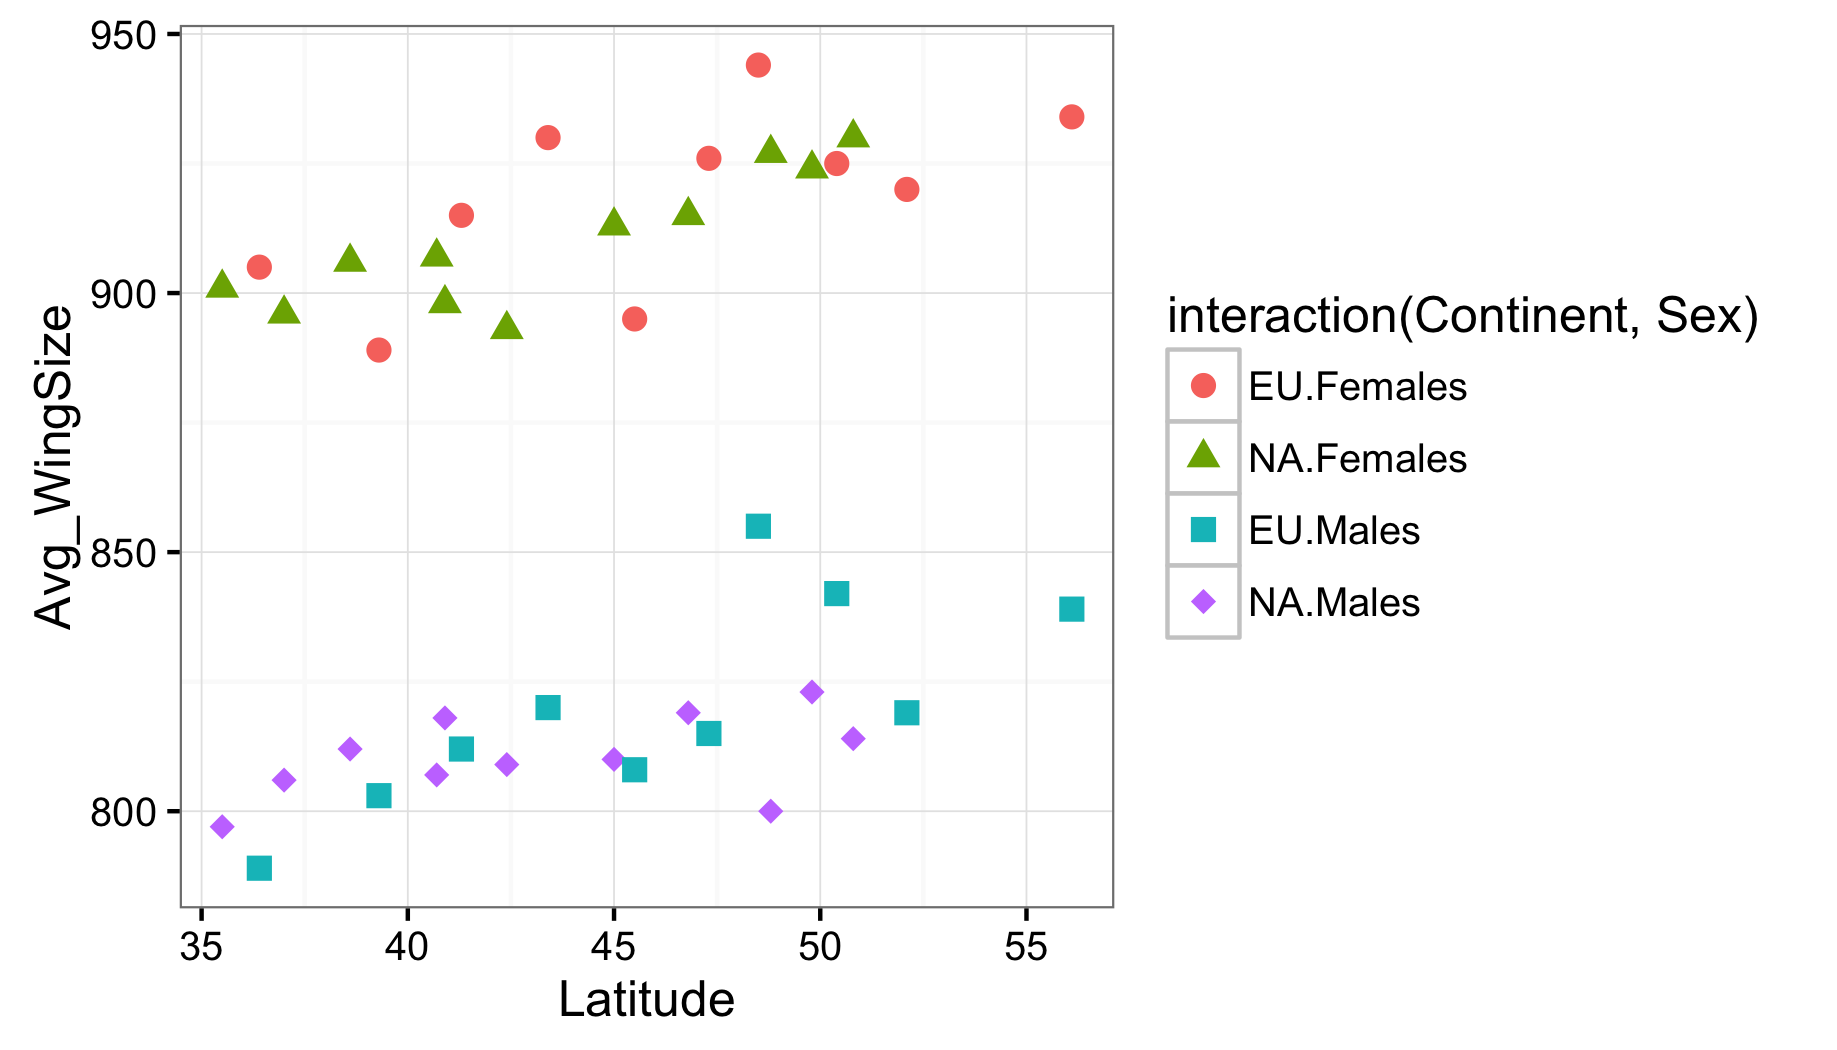
\includegraphics[width=4.25in]{3a.png}
	\caption{Scatterplot of average wing size vs latitude, by continent and sex.}
	\label{fig:3a}
\end{figure}



\part \textit{Construct a multiple linear regression model with wing size as the response, with latitude as a linear explanatory variable, and with indicator variables to distinguish the sexes and continents. As there are four groups, you will want to have three indicator variables: the continent indicator, the sex indicator, and the product of the two. Construct the model in such a way that one parameter measures the difference between the slopes of the wing size versus latitude regressions of NA and EU for males, one measures the difference between the NA–EU slope difference for females and that for males, one measures the difference between the intercepts of the regressions of NA and EU for males, and one measures the difference between the NA–EU intercepts' difference for females and that for males.} \todo{part b}






\end{parts}


\titledquestion{\ramsey 9.20}




\titledquestion{\ramsey 10.19}




\titledquestion{\ramsey 10.28}




\end{questions}

\listoftodos

\end{document}